\chapter{Voorstudie}
\section{Inleiding}
Dit hoofdstuk geeft informatie over de voorstudie dat was gedaan voordat er begonnen kon worden aan de implementatie. De volgende hoofdstukken worden beschrevenhardware validatie en communicatie. Uit deze twee delen wordt een conclusie getrokken om een robuuste applicatie te ontwikkelen die voldoet aan de volgende twee deelvragen:
\begin{enumerate}
	\item Hoe kan er een robuuste  communicatie gecreëerd worden tussen het hoofdsysteem en Satellite?
	\item Welke stappen zijn er nog om alle IO porten te testen van de Satellite?
\end{enumerate}

\section{Hardware validatie}
\subsection{Inleiding}
Elke nieuwe hardware wat aan Satellite wordt geleverd zal door Sensor Maritime moeten gevalideerd moeten worden dit betekend dat hiervoor een testplan ontwikkeld moet worden. Er zal als eerst beschreven worden welke porten er getest moet worden en hoe deze getest gaan worden en de uiteindelijke verwachte resultaat. De volgende type porten worden besproken. Ten eerste zal er gekeken worden naar DIP schakelaars, digitale output, analoge input, relay en uiteindelijk seriele communicatie. \newline

\noindent De Satellite heeft verschilllende porten porten zijn die gebruikt kan worden. Elke type port wordt beschreven in de volgende hoofdstukken. In deze hoofdstukken wordt beschreven wat de port moet doen en hoe dit getest gaat worden en uiteindelijk wat het verwachte resultaat is.

\subsection{DIP switch}
\subsubsection{Porten}
Een DIP switch bestaat uit een aantal schakelaars die je kan of uit kan zitten \autocite{DIP}. Op de Satellite is er een DIP switch aan bord, die acht schakelaar is heeft. Zeven van de acht worden op het moment gebruikt. Het volgende tabel \ref{tab:hw_val_dip} geeft aan wat de acties zijn als je de schakelaar aan of uit zet. De eerste drie van de schakelaars worden gebruikt als configuratie voor andere porten die worden beschreven in hoofdstuk \ref{Analog Input Signaal}. De laatste vier schakelaars zetten een specifiek pin van de microcontroller hoog of laag.
\begin{table}[h!]
	\caption{DIP switch porten die gevalideerd moeten worden}
	\begin{tabular}{llllp{10cm}}
	\toprule
	\textbf{Naam} & \textbf{GPIO} & \textbf{Pin} & \textbf{IO} & \textbf{Beschrijving}	\\ \toprule
	PU1		& -			& - 	& -    		& Verandert de analog input 1 voltage tussen 0 en 24V	\\
	-		& -			& - 	& -    		& Wordt niet gebruikt.								\\
	PU2		& -			& - 	& -    		& Verandert de analog input 2 voltage tussen 0 en 24V	\\
	PU3		& -			& - 	& -    		& Verandert de analog input 3 voltage tussen 0 en 24V	\\
	ADD0 	& 3			& 10	& Input		& Zet de pin hoog of laag, aan de hand van of het aan staat of niet.		\\
	ADD1 	& 3			& 11	& Input		& Zet de pin hoog of laag, aan de hand van of het aan staat of niet.		\\
	ADD2 	& 3			& 12	& Input		& Zet de pin hoog of laag, aan de hand van of het aan staat of niet.		\\
	ADD3 	& 3			& 0 	& Input		& Zet de pin hoog of laag, aan de hand van of het aan staat of niet.		\\ \bottomrule
	\end{tabular}
	\label{tab:hw_val_dip}
\end{table}
\newpage

\subsubsection{Testplan}
De eerste drie schakelaars worden anders getest in vergelijking met de laatste vier. De laatste vier schakelaars maken vier leds branden die op Satellite zitten. In het volgende tabel \ref{tab:hw_val_dip_testplan} is een overzicht van het testplan:
\begin{table}[h!]
	\caption{DIP switch porten testplan}
	\begin{tabular}{lp{14.5cm}}
	\toprule
	\textbf{Naam} 	& \textbf{Verwachte resultaat} \\ \toprule
	PU1				& Als het aan gezet wordt de range van de analoge input 1 verhoogt naar 24 volt, dit verhoogt de waarde wat de microcontroller leest, de waarde wordt laten zien op een GUI.\\
	-				& Wordt niet getest. \\
	PU2				& Als het aan gezet wordt de range van de analoge input 2 verhoogt naar 24 volt, dit verhoogt de waarde wat de microcontroller leest, de waarde wordt laten zien op een GUI.\\
	PU3				& Als het aan gezet wordt de range van de analoge input 3 verhoogt  naar 24 volt, dit verhoogt de waarde wat de microcontroller leest, de waarde wordt laten zien op een GUI. \\
	ADD0 			& Zet 3.3V op de pin van de microcontroller, als de microcontroller 3.3V detecteert zet het led 0 aan.\\
	ADD1 			& Zet 3.3V op de pin van de microcontroller, als de microcontroller 3.3V detecteert zet het led 1 aan.\\
	ADD2 			& Zet 3.3V op de pin van de microcontroller, als de microcontroller 3.3V detecteert zet het led 2 aan.\\
	ADD3 			& Zet 3.3V op de pin van de microcontroller, als de microcontroller 3.3V detecteert zet het led 3 aan.\\ \bottomrule
	\end{tabular}
	\label{tab:hw_val_dip_testplan}
\end{table}

\newpage
\subsection{Digital output signaal}
De digitale output signaal kan alleen hoog of uit gezet worden, dit betekent dat het geen input modus heeft. De Satellite heeft vier digitale output porten die op 24V of 0V gezet kan worden. Het volgende tabel geeft een overzicht \ref{tab:hw_val_dio}.
\subsubsection{Porten}
\begin{table}[h!]
	\caption{Digital output signalen die gevalideerd moeten worden}
	\begin{tabular}{llllp{10cm}}
	\toprule
	\textbf{Naam} & \textbf{GPIO} & \textbf{Pin} & \textbf{IO} & \textbf{Beschrijving}				 	\\ \toprule
	D1			& 1			& 6    	& Output	& Digital output signaal, op deze pin komt 24V of 0V. \\
	D2			& 1			& 7    	& Output	& Digital output signaal, op deze pin komt 24V of 0V. \\
	D3			& 3			& 3    	& Output	& Digital output signaal, op deze pin komt 24V of 0V. \\
	D4			& 3			& 2   	& Output	& Digital output signaal, op deze pin komt 24V of 0V. \\ \bottomrule
	\end{tabular}
	\label{tab:hw_val_dio}
\end{table}

\subsubsection{Testplan}
Alle digitale output porten voeren dezelfde actie. Het doel is dat als een LED verbonden is met de port dat die dan aan of uit gaat om de 1 seconden.
\begin{table}[h!]
	\caption{Digital output signalen testplan}
	\begin{tabular}{lp{14.5cm}}
	\toprule
	\textbf{Naam} 	& \textbf{Verwachte resultaat} \\ \toprule
	D1	&	Als op de pin 24V staat gaat het lampje aan, en bij 0V uit gaat het uit. Dit gebeurt om 1 seconden. \\			
	D2	&	Als op de pin 24V staat gaat het lampje aan, en bij 0V uit gaat het uit. Dit gebeurt om 1 seconden. \\			
	D3	&	Als op de pin 24V staat gaat het lampje aan, en bij 0V uit gaat het uit. Dit gebeurt om 1 seconden. \\			
	D4	&	Als op de pin 24V staat gaat het lampje aan, en bij 0V uit gaat het uit. Dit gebeurt om 1 seconden. \\ \bottomrule
	\end{tabular}
	\label{tab:hw_val_dio_testplan}
\end{table}

\newpage
\subsection{Analog input signaal} \label{Analog Input Signaal}
\subsubsection{Porten}
De analog signalen kan alleen uitgelezen worden, dit betekent dat het alleen een input modus heeft. De Satellite heeft drie analoge input porten aan bord. In het volgende tabel wordt een overzicht gegeven \ref{tab:hw_val_ai}.
\begin{table}[h!]
	\caption{Analog input signalen die gevalideerd moeten worden}
	\begin{tabular}{llllp{9cm}}
	\toprule
	\textbf{IO} & \textbf{GPIO} & \textbf{Pin} & \textbf{Input/Output} & \textbf{Beschrijving}			\\ \toprule
	AI1			& 14		& 2    	& Input		& Analoge input signaal van 0 tot 24 volt.					\\
	AI2			& 14		& 3    	& Input		& Analoge input signaal van 0 tot 24 volt.					\\
	AI3			& 14		& 12   	& Input		& Analoge input signaal van 0 tot 24 volt.					\\  \bottomrule
	\end{tabular}
	\label{tab:hw_val_ai}
\end{table}
\subsubsection{Testplan}
Aan de hand wat is beschreven zal er gebruik gemaakt worden van de DIP schakelaars PU1, PU2, en PU3 om de analoge input te testen. De microcontroller heeft een 12 bit Analog to Digital Converter (ADC) \autocite{microcontroller}. Dit betekent dat het bereik van analoge input porten van 0 tot 4096 ($2^{12}$) is. Dus bij 24 volt zal de microcontroller ongeveer 4096 in lezen, het getal kan af en toe lager zijn in ver band met ruis. Bij 0 volt zal de microcontroller 0 in lezen. PU1, PU2, PU3 zet het analoge bereik tussen 3,3 volt en 24 volt. Dit betekent als PU1, PU2 of PU3 uitstaan dat de maximale bereik 3,3 volt is en als het aan staat is de bereik 24 Volt. Om het bereik te testen zal er gebruikt gemaakt worden van een Graphical User Interface (GUI). De microcontroller zal om 100 microseconden de analoge input omzetten naar een digitale waarden en dit opsturen over UDP. Hiermee kan geverifieerd worden dat als de DIP schakelaars uitstaan dat het bereik van de waarden van 0 tot 1100 gaan. Als de DIP schakelaars aan staan dan zal het bereik zijn van 0 tot 4096. Hieronder is een overzicht van hoe de analoge input porten gevalideerd worden \ref{tab:hw_val_ai_testplan}.
\begin{table}[h!]
	\caption{Testplan voor de analoge input signalen}
	\begin{tabular}{lp{14.5cm}}
	\toprule
	\textbf{Naam} 	& \textbf{Verwachte resultaat} \\ \toprule
	AI1			& Als de schakelaar PU1 van de schakelaar aangezet wordt dan zal de data bereik op de graphical user interface aangepast worden naar 0 tot 4096. Als het dip schakelaar uit staat dan zal de bereik maar van 0 tot 1100 gaan.\\
	AI2			& Als de schakelaar PU1 van de schakelaar aangezet wordt dan zal de data bereik op de graphical user interface aangepast worden naar 0 tot 4096. Als het dip schakelaar uit staat dan zal de bereik maar van 0 tot 1100 gaan.\\
	AI3			& Als de schakelaar PU1 van de schakelaar aangezet wordt dan zal de data bereik op de graphical user interface aangepast worden naar 0 tot 4096. Als het dip schakelaar uit staat dan zal de bereik maar van 0 tot 1100 gaan.\\  \bottomrule
	\end{tabular}
	\label{tab:hw_val_ai_testplan}
\end{table}


\subsection{Relay}
\subsubsection{Porten}
Er is een relay verbonden aan de microcontroller. Een relay is een mechanisch apparaat dat een elektrische connectie maakt tussen twee of meer punten op reactie van de microcontroller. Als er 3,3 volt op de relay gezet wordt zal de relay sluiten en bij 0 volt zal het weer openen gaan. Omdat het mechanisch is moet je dit ook kunnen horen \autocite{relay}. Hieronder is een overzicht van de relay \ref{tab:hw_val_relay}.

\begin{table}[h!]
	\caption{Relay signaal die gevalideerd moeten worden}
	\begin{tabular}{llllp{9cm}}
	\toprule
	\textbf{IO} & \textbf{GPIO} & \textbf{Pin} & \textbf{Input/Output} & \textbf{Beschrijving}			\\ \toprule
	Relay		& 3 & 1   	& Output		& Een mechanische apparaat was dicht of opengaat aan de hand of er 3,3 volt of niet op staat.	\\ \bottomrule
	\end{tabular}
	\label{tab:hw_val_relay}
\end{table}
\subsubsection{Testplan}
De relay geeft bij het sluiten en het openen van de mechanische connectie een luid geluid wat op normale afstand van het apparaat te horen moet zijn. Het testplan van de relay wordt dan ook op geluid gedaan. De relay zal dan voor vijf seconden aan gaan, en vervolgens weer voor vijf seconden uitgaan. Hieronder is een overzicht van de relay testplan \ref{tab:hw_val_relay_testplan}.

\begin{table}[h!]
	\caption{Testplan voor de relay}
	\begin{tabular}{lp{14.5cm}}
	\toprule
	\textbf{Naam} 	& \textbf{Verwachte resultaat} \\ \toprule
	Relay			& De microcontroller zet de pin van de relay voor vijf seconden hoog, als dit gebeurt hoor je een klik te horen. Na vijf seconden zal deze pin weer laag gezet worden, dit moet ook gehoord kunnen worden.\\  \bottomrule
	\end{tabular}
	\label{tab:hw_val_relay_testplan}
\end{table}
\newpage

\subsection{Serieel Communicatie}
\subsubsection{Porten}
De Satellite heeft verschillende porten voor seriele communicatie aanbord. De seriele communicatie middelen zullen gebruikt worden voor communicatie met een eindsysteem of sensoren. Sommige sensoren die Sensor Maritime gebruiken sturen de gegevens via seriele communicatie over. Omdat het zoveel functionaliteiten heeft zal dit grondig getest moeten worden. Satellite heeft verschillende varianten van seriele communicatie, ten eerste zijn er twee UART verbindingen, een RS232 verbinding, en uiteindelijk een RS422 communicatie lijn. \newline

\noindent UART staat voor Universal asynchronous receiver-transmitter. UART stuurt asynchroon data over dit betekent dat er geen klok signaal is die data synchroon maakt. UART wordt universeel genoemd omdat het geconfigureerd om verschillende seriele protocollen te ondersteunen. In plaats van een klok signaal wordt er gebruikt gemaakt van een start bit en een stop bit. Data wordt verstuurd via UART via de gebruiker gespecificeerd frequentie, dit wordt ook wel baudrate genoemd, baudrate wordt gespecificeerd als in bits per seconden (bps) \autocite{UART}. \newline

\noindent RS-232 is anders opgebouwd dan UART. RS-232 is een standaard gedefineerd signaal tussen twee apparaten, waar de signaal naam, doel, spanningniveau en pinnen zijn gedefineerd zijn. Een belangrijk verschil tussen RS-232 en UART is dat de spanningniveau hoger en negatief kan zijn. Het voltage bereik van RS-232 gaat -12 volt tot 12 volt \autocite{RS232}. \newline

\noindent RS-422 is weer een andere vorm van seriele communicatie en heeft kenmerken van RS-232. Het verschil tussen RS-232 en RS-422 is dat het voor de communicatie vier lijnen gebruikt (RX-, RX+, TX+, TX-). Met de vier communicatielijnen kan er full duplex gecommuniceerd worden. Full duplex communicatie betekent dat er twee of meer apparaten in beide richting kan communiceren (ontvangen en verzenden op hetzelfde moment) \autocite{FullDuplex}. RS-232 heeft half-duplex dit houdt in dat via RS-232 alleen handeling gedaan kan worden, bijvoorbeeld eerst ontvangen en dan pas verzenden. \autocite{RS422}. \newpage

\noindent In het volgende tabel \ref{tab:hw_val_serieel}wordt een overzicht gegeven van de seriele communicatie die verbonden zijn op de microcontroller. Voor de RS-422 communicatie is alleen twee communicatielijnen aangegeven, omdat dit zo verbonden is op de microcontroller. De Rx+, RX- en TX+, TX- lijnen worden samengevoegd door een chip en dan verbonden naar de microcontroller.
\begin{table}[h!]
	\caption{Seriele communicatie porten die gevalideerd moeten worden}
	\begin{tabular}{llllp{9cm}}
	\toprule
	\textbf{IO} & \textbf{GPIO} & \textbf{Pin} & \textbf{Input/Output} & \textbf{Beschrijving}	\\ \toprule
	UART RX		& 5			& 0    	& Input		& Seriele communicatie ontvangst lijn.			\\
	UART TX		& 5			& 1    	& Output	& Seriele communicatie versturen lijn.			\\
	RS-232 RX	& 3			& 7    	& Input		& Seriele communicatie ontvangst lijn.			\\
	RS-232 TX	& 3			& 8    	& Output	& Seriele communicatie versturen lijn.			\\
	RS-422 RX	& 6			& 3    	& Input		& Seriele communicatie ontvangst lijn.			\\
	RS-422 TX	& 3			& 13   	& Output	& Seriele communicatie versturen lijn.			\\
	UART 2 RX	& 4			& 6    	& Input		& Seriele communicatie ontvangst lijn.			\\
	UART 2 TX	& 4			& 7   	& Output	& Seriele communicatie versturen lijn.			\\ \bottomrule
	\end{tabular}
	\label{tab:hw_val_serieel}
\end{table}

\subsubsection{Testplan}
Om de seriele communicatie te testen wordt er gebruikt gemaakt van GUI. Deze GUI vraagt de om gebruikers input hier in kan de gebruiker een tekst schrijven en dit wordt opgestuurd. De tekst heeft een limiet van maximaal 32 karakters. Er zal hier automatisch een newline karakter toegevoegd worden zodat de microcontroller weet dat dit het einde van het gebruikers bericht is. Het bericht wordt opgestuurd naar de microcontroller en zal de data verwerken. De microcontroller zal dan een antwoord geven als volgt, ten eerste zal de microcontroller vertellen welke variant van communicatie is gebruikt en daarna zal het toevoegen wat de microcontroller ontvangen heeft van de gebruiker. Hieronder is een overzicht \ref{fig:testplanserieel} van hoe het testplan zal werken.

\begin{figure}[h!]
	\caption{Testplan seriele communicatie}
	\label{fig:testplanserieel}
	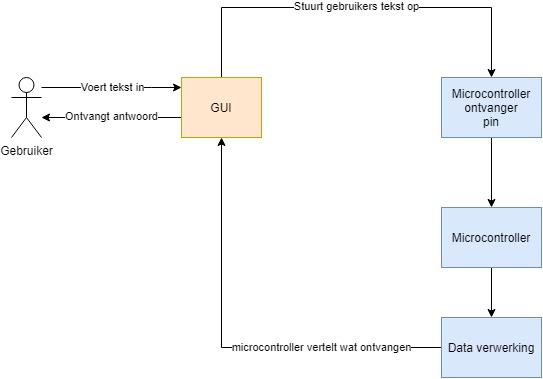
\includegraphics[width=0.5\linewidth]{voorstudie/testplan/Serieel.jpg}
\end{figure}



\newpage
\section{Communicatie}
\subsection{Inleiding}
De Satellite heeft verschillende communicatie middelen, onderanderen ethernet, CAN Bus en serieel communicatie. Alle deze vormen van communicatie moeten voldoen aan het volgende deelvraag: \textbf{Hoe kan er een robuuste communicatie gecreëerd worden tussen het hoofdsysteem en Satellite?}. Er moet gekeken worden hoe dit stabiel en robuust gedaan kan worden.

\subsection{Ethernet}
Satellite heeft standaard ethernet support dit betekent dat via een ethernet kabel naar een end device gecommuniceerd kan worden. Dit wordt alleen via de User Datagram Protocol (UDP) internet protocol gedaan. UDP is een standaard methode om data te versturen tussen twee systemen \autocite{CloudFlareUDP}. \newline

\noindent Om een betrouwbare communicatie te creëren zal er gebruikt gemaakt worden van een library. Een eigen library hiervoor te schrijven zal veel tijd kosten en is buiten het scoop van het project. Hiervoor zijn er een aantal opties om uit te kiezen: lwIP, uIP, FreeRTOS TCP/IP. Voor deze drie libraries wordt er gekeken wat de pluspunten en negatieve punten zijn:

\subsubsection{LWiP}
LWip (Lightweight TCP/IP) is een open source implementatie van TCP/IP stack dat zicht focust minder geheugen te gebruiken, maar nog steeds alle grote features te hebben. lwIP zorgt ervoor dat er makkelijk connectie gemaakt kan worden tussen verschillende systemen \autocite{LWIP}. Hieronder is een overzicht gemaakt \ref{tab:lwipoverzicht} met de pluspunten en de negatieve punten van LwIP.

\begin{table}[h!]
	\caption{Pluspunten en minpunten van LwIP}
	\begin{tabular}{p{8cm}p{8cm}}
	\toprule
	Pluspunten & Minpunten \\ \midrule
	Een kleine TCP/IP implementatie	met snelle performance. \autocite{lwipuip}	&  Niet geschikt voor hele kleine embedded systemen \autocite{lwipuip}         \\
																				&           \\
			   																	&           \\
			   																	&           \\ \bottomrule
	\end{tabular}
	
	\label{tab:lwipoverzicht}
\end{table}

\newpage
\subsubsection{UIP}
Hieronder is een overzicht \ref{tab:uipoverzicht} van de pluspunten en minpunten van UIP.
\begin{table}[h!]
	\caption{Pluspunten en minpunten van UIP}
	\begin{tabular}{p{8cm}p{8cm}}
	\toprule
	Pluspunten & Minpunten \\ \midrule
	Ontwikkelt voor systemen met echte beperkte snelheiden en geheugen \autocite{lwipuip} &           \\
			   															&           \\
			   															&           \\
			   															&           \\ \bottomrule
	\end{tabular}
	
	\label{tab:uipoverzicht}
\end{table}

\subsubsection{Conclusie}

\newpage
\subsection{CAN communicatie}
CAN is een groot onderdeel van de Sensor Maritime infrastructuur. De CAN communicatie wordt gebruik om te kunnen communiceren met het hoofdsysteem genaamd het hub. Hiervoor wordt een master en slave configuratie gebruikt. Het hub is de master en de Satellite en andere eindsystemen zullen dan de slave zijn. De master bepaalt hoe een slave apparaat zich gaat gedragen. CAN staat voor controlled area network, en maakt gebruik van een broadcast systeem. Dit betekent dat alle eindsystemen alle berichten ontvangen, De master kan niet specifiek naar een slave data sturen \autocite{can}. \newline

\noindent Sensor Maritime heeft een eigen protocol ontwikkeld wat gebouwd is op het CAN Bus. Dit zal deels aangepast moeten worden om de Satellite sensoren te kunnen ondersteunen. De huidige protocol wat gebruikt wordt is in afbeelding \ref{fig:canprotocol} te zien. Het protocol is opgebouwd uit blokjes wat uit 1 of 2 bytes bestaat. In tabel \ref{tab:cansensorprotocol} wordt beschreven wat de taak is van het blokje. 
\begin{figure}[h!]
	\label{fig:canprotocol}
	\caption{Sensor Maritime CAN protocol}
	
\includegraphics[width=\linewidth]{voorstudie/communicatie/can.png}
\end{figure}

\begin{table}[h!]
	\caption{Sensor Maritime CAN protocol opbouw}
	\label{tab:cansensorprotocol}
	\begin{tabular}{p{1.5cm}p{10.5cm}p{3cm}}
	\toprule
	\textbf{Blok} & \textbf{Beschrijving} & \textbf{Waarde}\\ \midrule
	S1		& Het eerst start byte, dit geeft het start aan van het CAN bericht en wordt gebruikt voor herkenning, dit is een vaste waard.	& 0x40 \\
	S2		& Het tweede start byte, dit geeft het start aan van het CAN bericht en wordt gebruikt voor herkenning, dit is een vaste waard. & 0x02 \\
	Dest	& Deze byte beschrijft voor wie het bericht bedoeld is.		& Verschillend per apparaat. \\
	Src		& Deze byte beschrijft van welke apparaat het bericht komt	& Verschillend per apparaat.\\ 
	Flag	& Dit geeft aan wat voor type bericht het is.             & 0 voor commando \\ 
			& & 1 voor request \\ 
	DLC		& DLC is een afkorting voor Data Length Code.             & \\ 
	Payload	& De data die aan de hand de flag. & Verschillend per bericht\\
	CRC		& CRC staat voor Cyclic redundancy check, dit beschrijft hoe groot het bericht is wat verstuurd word, Hiermee kan de ontvanger valideren of het juiste is ontvangen. & Verschillend per bericht\\ \bottomrule
	\end{tabular}
\end{table}

\subsubsection{Probleemstelling}
Om het volgende deelvraag te kunnen beantwoorden zal er een aanpassing gemaakt moeten worden aan de bestaande CAN protocol van Sensor Maritime. De deelvraag wat beantwoord moet worden luid als volgt \textbf{Hoe kan er een robuuste  communicatie gecreëerd worden tussen het hoofdsysteem en Satellite?}